\documentclass[12pt]{article}
\usepackage[spanish]{babel}
\usepackage[utf8]{inputenc}

% Extras
\usepackage{url}
\usepackage{hyperref}
\usepackage{float}  % H
\usepackage{amsmath}

% Imágenes
\usepackage{graphicx}
\graphicspath{{images/}}

% Cambio de la fuente de las secciones
\usepackage{setspace}
\usepackage{sectsty}
\allsectionsfont{\normalfont\scshape}

% Configuración página
\usepackage{vmargin}
\setmarginsrb{3 cm}{2.5 cm}{3 cm}{2.5 cm}{1 cm}{1.5 cm}{1 cm}{1.5 cm}
\usepackage{fancyhdr}
\pagestyle{fancy}
\lhead{}
\cfoot{\thepage}

% Configuración portada
\title{Proyecto de Clasificación: Limpieza, Transformación y Creación de un Primer Modelo}			                % Título
\author{Daniel González Alonso\\		% Autor
        Joshua Miguel González Santana\\
		Javier Estefanía González}
\date{\today}							% Fecha

\makeatletter
\let\thetitle\@title
\let\theauthor\@author
\let\thedate\@date
\makeatother


%%%%%%%%%%%%%%%%%%%%%%%%%%%%%%%%%%%%%%%%%%%%%%%%%%%%%%%%%%%%%%%%%%%%%%%%%%%%%%%%%%%%%%%%%
\begin{document}

%%%%%%%%%% PORTADA %%%%%%%%%%
\begin{titlepage}
	\centering
    \vspace*{0.25 cm}
	
	\doublespacing
	\textsc{\LARGE Máster Universitario en Inteligencia de Negocio y Big Data en Entornos Seguros}\\[0.5 cm]
	\singlespacing
	\textsc{\large Técnicas de Aprendizaje Automático Escalables}\\[0.5 cm]
	
	\rule{\linewidth}{0.2 mm}\\[0.4 cm]
	\textsc{\huge \bf \thetitle}\\
	\rule{\linewidth}{0.2 mm}\\[2.5 cm]
	
	\begin{minipage}{0.6\textwidth}
		\begin{flushleft} \large
			\emph{Autores:}\\
			\begin{itemize}
            	\item[] \theauthor
            \end{itemize}
		\end{flushleft}
	\end{minipage}~
	\begin{minipage}{0.3\textwidth}
		\begin{flushright} \large
		\end{flushright}
	\end{minipage}\\[6 cm]
	{\large \thedate}\\[2 cm]

	\vfill	
\end{titlepage}

%%%%%%%%%% INDICE %%%%%%%%%%
\tableofcontents
\pagebreak

%%%%%%%%%%%%%%%%%%%%%%%%%%%%%%%%%%%%%%%%%%%%%%%%%%%%%%%%%%%%%%%%%%%%%%%%%%%%%%%%%%%%%%%%%
%%%% Introducción %%%%
\section{Introducción}
Este documento es el segundo de una serie de entregables que forman parte del \textbf{Proyecto de clasificación} de la asignatura Técnicas de Aprendizaje Automático Escalables, que consistirá, en último término y de acuerdo con el enunciado, en comparar el rendimiento de varios clasificadores de la biblioteca de Spark ML.\\

En este segundo entregable se va a trabajar sobre el conjunto de datos \textit{NYC Taxi Trip Duration} \cite{kaggle} que se describía en la primera parte. Esta entrega se divide en varias secciones, primeramente se va a llevar a cabo una división del conjunto de datos en dos subconjuntos, uno de entrenamiento y otro de prueba. Posteriormente, se describirá la fase de limpieza de datos. Después se tratarán las transformaciones necesarias llevadas a cabo sobre el conjunto de datos. Finalmente, se llevará a cabo un modelo y se evaluará su comportamiento.\\

%%%% Conjuntos de entrenamiento y prueba %%%%
\section{Conjuntos de Entrenamiento y Prueba}\label{cap2}
Para poder entrenar y probar el modelo es necesario separar el conjunto de datos inicial, almacenado en el fichero \texttt{train.csv}, en dos subconjuntos de datos:

\begin{itemize}
    \item Conjunto de entrenamiento \textit{train}, empleado para crear el modelo.
    \item Conjunto de prueba \textit{test}, empleado para probar el modelo.
\end{itemize}

Ambos conjuntos de datos serán sometidos al mismo pre-procesamiento, pero por separado, para evitar que se haga un uso indebido del conjunto de datos de prueba.\\

La separación del conjunto de datos original ha sido llevada a cabo en proporción $2/3$ para el conjunto de entrenamiento y $1/3$ para el conjunto de prueba, con los datos escogidos aleatoriamente empleando la función \texttt{randomSplit} de la librería ML de Scala.\\

\newpage

%%%% Limpieza de datos %%%%
\section{Limpieza de Datos}\label{cap3}
En el conjunto de datos original, con un total de 1458644 registros, no existía ninguno con valores nulos, así que no se ha encontrado ningún atributo que haya tenido que ser reemplazado o registro que haya sido descartado.\\

Lo que si se ha hecho ha sido limpiar valores atípicos. Durante la exploración de los datos se observó que hubo dos fechas que convenía tratar, por un lado el 1 de Julio de 2016, ya que al tratarse del último día del conjunto de datos, el número de ejemplos era muy pequeño, y el día 23 de Enero de 2016, ya que ese día hubo también muy pocos tránsitos debido a un temporal de nieve que bloqueó la ciudad. Se ha decidido eliminar los tránsitos de ambos días para evitar que estos outliers afecten al modelo.\\

Esta limpieza se ha aplicado por separado tanto al conjunto de entrenamiento como al de prueba. El número total de instancias eliminadas del conjunto de prueba debido a valores nulos (NTAIE) ha sido de 0, mientras que el número de instancias eliminadas por ser valores atípicos (NTOE) ha sido de 632. Esto nos da una tasa de no clasificados de:\\

\begin{equation}
    \textnormal{TNC} = \frac{\text{NTAIE} + \text{NTOE}}{\textnormal{tamaño conjunto de pruebas}} = \frac{0 + 632}{1458644} = 0.001274128
    \label{eq:tasa-no-clasificados}
\end{equation}

%%%% Transformación de datos %%%%
\section{Transformación de Datos}
En esta sección se describen las transformaciones realizadas sobre los atributos para poder obtener posteriormente el modelo, junto con las transformaciones llevadas a cabo para obtener las columnas ``features'' y ``labels''.\\

\subsection{Transformación de Atributos para el Modelo}

Las transformaciones llevadas a cabo han sido las siguientes:

\begin{itemize}
    \item Cómo se describía en la entrega anterior, el atributo \texttt{store\_and\_fwd\_flag} es una bandera que puede tomar dos valores (binario), \textit{Y} o \textit{N}, es decir, se tarta de un valor categórico, pero cuyos valores no tienen ningún orden. Por ello, para transformar el valor a tipo \texttt{Double} se ha decidido emplear, primero una transformación de String a índice de clase empleando \texttt{StringIndexer} con el orden alfabético como índice, y después, la codificación 1 de k con el \texttt{OneHotEncoderEstimator}.
    \item Se ha definido la función \texttt{convertDates} con el fin de transformar los atributos que estaban almacenados como \texttt{DateTime} en formato \texttt{YYYY-MM-DD hh:mm:ss} (atributos \texttt{pickup\_datetime y dropoff\_datetime}) a diferentes columnas en las que se almacenan por separado el día de la semana con el que se corresponde el trayecto. Así como las horas, minutos y segundos (de inicio y fin de trayecto) en tipo \texttt{Double}. Los días de la semana, al tratarse de un valor categórico se han codificado empleando el StringIndexer con el número de la semana, y después se ha aplicado el \texttt{OneHotEncoderEstimator}. Se ha decidido no capturar por separado los días del mes, ni el mes en si, ya que el periodo en el que se capturaron los datos tan solo abarca los días entre Enero y Julio, por lo que no se detectarían cambios en el modelo debido a la estacionalidad.
    \item Se ha transformado la columna \texttt{trip\_duration}, la cual en el archivo de origen era de tipo numérico continuo (\texttt{Double}), mientras que ahora es un valor categórico binario, con las clases \texttt{short} y \texttt{long}. Estas clases se han asignado calculando la mediana de los valores que tomaba este atributo, la cual ha sido de $663.0$. Si el valor del trayecto es superior a la mediana de la columna, se ha sustituido por \texttt{long}, y si por el contrario, la duración ha sido inferior a la mediana, tomará el valor \texttt{short}.
\end{itemize}

Todas estas transformaciones se han realizado por separado sobre los conjuntos de entrenamiento y prueba para que tengan el mismo formato. Pero las transformaciones que han necesitado de un estimador como el \textit{OneHotEncoder} sólo se han ajustado (\textit{fit}) sobre el conjunto de entrenamiento, y después se han aplicado también al conjunto de prueba.

\subsection{Transformación para obtener Features y Labels}
Por último, durante la fase de transformación se han obtenidos dos columnas, una llamada \textit{features} con el vector de características de entrada para los modelos de Scala ML, y otra llamada \textit{labels} con la columna de la etiqueta de clase.

\begin{itemize}
    \item Para obtener \textit{features} se han empleado todas las columnas a excepción de \texttt{trip\_duration}, y se las ha aplicado el \textit{transformer} \texttt{VectorAssembler} directamente, ya que llegados aquí todas estas columnas ya están con tipos \texttt{Double} o \texttt{Vector}.
    \item Para obtener la columna \textit{label} se ha empleado la columna \texttt{trip\_duration}, que será nuestra clase. A esta columna, ahora en almacenada como \texttt{String}, ha habido que transformarla a tipo \texttt{Double} empleando \texttt{StringIndexer}.
\end{itemize}

Al igual que las transformaciones del apartado anterior, estas se han realizado por separado sobre los conjuntos de entrenamiento y prueba.

%%%% Creación del modelo %%%%
\section{Creación del Modelo}

En esta sección se seguirán los pasos necesarios para ajustar y generar un primer árbol de decisión binario usando la biblioteca Spark ML. Existen una serie de parámetros sobre los que actuar con el fin de obtener un mejor ajuste del modelo.

\subsection{Entrenamiento y Validación}
Antes de crear el modelo final se ha realizado, de acuerdo con la aproximación propuesta en el enunciado del entregable, una segunda partición de los datos, para ser utilizado con distintos fines. Esta segunda partición se ha realizado sobre el conjunto de datos de entrenamiento (\texttt{train}) que se había obtenido tras la primera escisión, descrita en la sección \ref{cap2} de este documento.
\begin{itemize}
    \item En primer lugar, se crea una partición con el 66.6\% de los datos de \texttt{train}, que será utilizada en esta misma sección para entrenar diferentes modelos con el fin de ajustar los parámetros que intervienen en el modelo final a utilizar. Estos modelos se validarán con el 33.3\% de datos restantes, obteniendo su correspondiente tasa de error que se empleará para tomar la decisión sobre cuales son los mejores parámetros para usar.
    \item Una vez la decisión de los parámetros a utilizar haya sido tomada, todo el conjunto definido originalmente como \texttt{train} se destinará al entrenamiento del modelo final, este modelo se encuentra descrito en la sección \nameref{cap5.2}.
\end{itemize}

Como se ha comentado anteriormente, para definir los parámetros del árbol final, se han generando múltiples árboles con diferentes parámetros y se ha calculado su correspondiente tasa de error. Esta tasa de error ha sido calculada como el número de errores de clasificación obtenido dividido por el tamaño del conjunto de prueba. En la siguiente tabla se muestran los parámetros empleados y los resultados obtenidos de estos árboles:

\begin{table}[H]
\centering
\begin{tabular}{|c|c|c|c|}
\hline
Id.    & maxProf    & maxBins  & tasa de error  \\ \hline
\texttt{testTree\_01}  &   3   & 10  & 0.382631  \\ \hline
\texttt{testTree\_02}  &   3   & 5   & 0.375108   \\ \hline
\texttt{testTree\_03}  &   4   & 5   & 0.316920   \\ \hline
\texttt{testTree\_04}  &   5   & 5   & 0.298965   \\ \hline
\texttt{testTree\_05}  &   6   & 5   & 0.294047   \\ \hline
\texttt{testTree\_06}  &   7   & 5   & 0.291005   \\ \hline
\texttt{testTree\_07}  &   8   & 5   & 0.267189   \\ \hline
\texttt{testTree\_08}  &   9   & 5   & 0.261618   \\ \hline
\texttt{testTree\_09}  &   9   & 32   & 0.267006   \\ \hline
\end{tabular}
\caption{Árboles generados para ajustar los parámetros}
\end{table}

A la vista de los resultados obtenidos, se puede observar que la configuración utilizando \texttt{maxProf = 9 , maxBins = 5} es la que menos tasa de error ha obtenido, por lo que será la finalmente seleccionada para nuestro primer modelo.

\subsection{Modelo Generado}\label{cap5.2}
Los parámetros finalmente empleados para generar el árbol de decisión final han sido los siguientes:

\begin{itemize}
    \item \texttt{Impureza}: Se selecciona la medida de impureza \texttt{gini}, por tener atributos de tipo numérico.
    \item \texttt{maxProf}: Se trata de la profundidad máxima que puede alcanzar el árbol. Un árbol demasiado profundo podría sobreajustar y uno menos profundo, podría no incluir un atributo necesario. Su valor por defecto es 5, se ha seleccionado el valor 9 para el modelo.
    \item \texttt{maxBins}: Se trata del número máximo de particiones de atributos continuos, a la vista de los resultado en la fase de validación, se ha seleccionado el valor 5 para el modelo.
    \item \texttt{minInstancesPerNode}: Cada atributo seleccionado induce una partición sobre la parte del 
    conjunto de entrenamiento que llega al nodo y detiene la construcción de la rama si ningún atributo genera particiones con más de \texttt{minInstancesPerNode} en cada rama. Valores pequeños favorecen el sobreajuste, su valor por defecto es 1, que se ha mantenido
\end{itemize}

Por último, cabe destacar que en el script de SCALA empleado para crear el modelo \texttt{trainTest.scala} se ha incluido un bloque de código que almacena el modelo generado tras su entrenamiento. Este bloque genera como salida un directorio en el lugar en el que se esté ejecutando, que incluye tanto datos, como metadatos del modelo.

\begin{figure}[H]
    \centering
    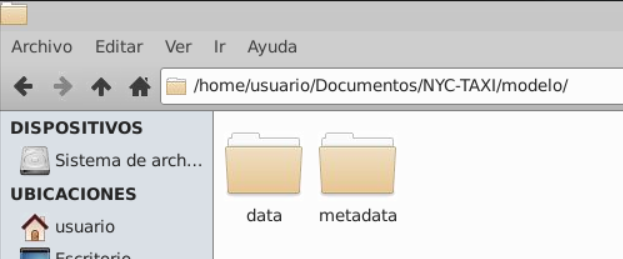
\includegraphics[width=0.9\textwidth]{guardado.png}
    \caption{Archivos guardados del modelo}
    \label{fig:guardado}
\end{figure}

Este modelo generado se adjunta también en la entrega.

%%%% Evaluación del modelo %%%%
\section{Evaluación del modelo}
En esta sección del documento se estima la tasa de error del modelo generado descrito en la sección anterior.\\

Dado que para este entregable no está permitido utilizar las métricas proporcionadas en las bibliotecas ML/MLlib, se ha generado un bloque de código \texttt{SCALA} para calcular esta tasa de error utilizando la aproximación propuesta en el enunciado de este entregable y que ya se ha comentado en apartados anteriores. En este código se recuentan los errores cometidos por el modelo y se comparan con el volumen de predicciones totales realizadas, obteniendo una tasa de error del modelo:

\begin{itemize}
    \item \texttt{Tasa de Error obtenida del modelo}: 0.26378
\end{itemize}

Como se justificaba anteriormente, en la sección \ref{cap3} de este entregable, se ha incluido de igual manera en el script el calculo de la tasa de no clasificados

\begin{itemize}
    \item \texttt{Tasa de no clasificados} \ref{eq:tasa-no-clasificados}: 0.001274
\end{itemize}

Coincidiendo con la definición para este valor, la tasa de no clasificados es de varios órdenes de magnitud menor que la tasa de error obtenida.\\

Además del script de entrenamiento \texttt{trainTest.scala}, se ha creado un script \texttt{loadModel.scala} que permite cargar el modelo generado en el apartado \nameref{cap5.2} y probarlo con el conjunto de datos que se quiera cambiando los parámetros \textit{PATH} y \textit{FILE} que se encuentran en la parte superior del script, mostrando la tasa de no clasificados y la tasa de error obtenida.\\

%%%% Esfuerzo %%%%
\section{Esfuerzo}

La distribución del esfuerzo realizado en el análisis, compresión, redacción y coordinación de este documento ha sido la siguiente:

\begin{table}[H]
\centering
\begin{tabular}{|c|c|c|}
\hline
Alumno         & Esfuerzo (Hr)    & Tanto por ciento  \\ \hline
\textit{Daniel Gonzalez Alonso}  &   13   & $33.3\%$      \\ \hline
\textit{Joshua M. González Santana}  & 13  & $33.3\%$      \\ \hline
\textit{Javier Estefanía González}  & 13  & $33.3\%$      \\ \hline
\end{tabular}
\caption{Carga de trabajo de los alumnos}
\end{table}

%%%% REFERENCIAS %%%%%
\section{Bibliografía}
\begin{thebibliography}{0}
	\bibitem{kaggle}
      Kaggle,
      \emph{New York City Taxi Trip Duration},
      \url{https://www.kaggle.com/c/nyc-taxi-trip-duration/code}
\end{thebibliography}

\end{document}
